% !TEX root = ../tex/4-4.tex
% 第4章：本文は青、補足は緑
\newcommand{\asmain}{%
    \setbeamercolor{frametitle}{fg=white,bg=main}%
    \setbeamercolor{structure}{fg=main}%
    \setbeamercolor{itemize item}{fg=main}%
    \setbeamercolor{itemize subitem}{fg=main}%
    \setbeamercolor{enumerate item}{fg=main}%
}
\newcommand{\assuppl}{%
    \setbeamercolor{frametitle}{fg=white,bg=examplecol}%
    \setbeamercolor{structure}{fg=examplecol}%
    \setbeamercolor{itemize item}{fg=examplecol}%
    \setbeamercolor{itemize subitem}{fg=examplecol}%
    \setbeamercolor{enumerate item}{fg=examplecol}%
}
% フレームタイトルの「補足」だけを□で囲む
\newcommand{\supplmark}{%
    \setlength{\fboxsep}{1.5pt}%
    \setlength{\fboxrule}{0.7pt}%
    \fbox{\textbf{補足}}%
}
\asmain


%=============================================
\assuppl
\begin{frame}{\supplmark：4.3から4.4へ（任意）}
    \begin{block}{ここまで}
        VE / VPの$\bm{f},g$から摂動核$p_t(\bm{x}_t\mid\bm{x}_0)$を導いた。
    \end{block}
    \begin{block}{ここから（スライド4.4＝論文4.5）}
        逆に、\textbf{累積摂動核を先に置く}見方を取る。\\
        Score SDEと変分DDPMをつなぎ、学習の直感をはっきりさせる。
    \end{block}
    \vfill
    \footnotesize
    初読ではスキップ可。学習目的に出てくる$p_t(\bm{x}_t\mid\bm{x}_0)$の「なぜ便利か」を埋める節。
\end{frame}
%=============================================
\assuppl
\begin{frame}{\supplmark：4.4 の位置づけ}
    \begin{block}{この節の役割（任意）}
        局所ノイズ注入ではなく、累積核$\alpha_t,\sigma_t$から前向き過程を見る
    \end{block}
    \begin{enumerate}
        \item 図4.8：局所SDEと累積核は同じアフィン過程の二面
        \item Score SDEへ：$\alpha_t,\sigma_t$から$f(t),g(t)$を復元（補題4.5.1）
        \item 変分/DDPMへ：逆条件付きと拡散損失を核から書く
        \item なぜ学習に効くか：信号とノイズの量が時刻で明示される
    \end{enumerate}
\end{frame}
%=============================================
\section{累積摂動核}
\assuppl
\begin{frame}{区切り：\supplmark\;累積摂動核}
    \tableofcontents[currentsection]
\end{frame}
%=============================================
\assuppl
\begin{frame}{\supplmark：局所注入ではなく累積核}
    DDPMは$p(\bm{x}_t\mid\bm{x}_{t-\Delta t})$、Score SDEは連続SDEで\\
    「局所的なノイズの足し方」から入ることが多い。
    \begin{exampleblock}{学習で本当に使うもの}
        累積摂動核$p_t(\bm{x}_t\mid\bm{x}_0)$である。\\
        DDPM損失や連続時間DSM（2.2.8）（4.3.1）にそのまま現れる。
    \end{exampleblock}
    そこで、局所注入から導くのではなく、\\
    \textbf{累積核を直接指定する}見方をとる。
\end{frame}
%=============================================
\assuppl
\begin{frame}{\supplmark：図4.8：同じ過程の二面}
    \centering
    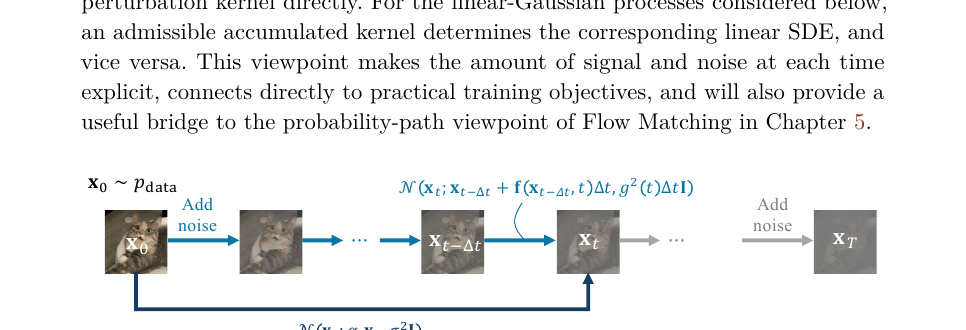
\includegraphics[width=\textwidth,height=0.62\textheight,keepaspectratio]{fig-4-8.png}
    \vfill
    \footnotesize
    上：微小ステップのノイズ注入。下：$\bm{x}_0$から$\bm{x}_t$へ一気に書く累積核。
\end{frame}
%=============================================
\assuppl
\begin{frame}{\supplmark：一般のアフィン前向き過程}
    \[
        p_t(\bm{x}_t\mid\bm{x}_0)
        :=
        \mathcal{N}\bigl(\bm{x}_t;\,\alpha_t\bm{x}_0,\,\sigma_t^{2}\bm{I}\bigr)
        \tag{4.5.1}
    \]
    等価なサンプリング：
    \[
        \bm{x}_t=\alpha_t\bm{x}_0+\sigma_t\bm{\epsilon},
        \qquad
        \bm{\epsilon}\sim\mathcal{N}(\bm{0},\bm{I})
    \]
    標準設定：$\alpha_0=1$、$\sigma_0=0$（時刻0はデータそのもの）。
\end{frame}
%=============================================
\assuppl
\begin{frame}{\supplmark：よくある確率パス}
    \begin{itemize}
        \item \textbf{VE（NCSN）}：$\alpha_t\equiv 1$、$\sigma_t$は時間とともに増加
        \item \textbf{VP（DDPM）}：$\alpha_t^{2}+\sigma_t^{2}=1$
        \item \textbf{線形補間}：$\alpha_t=1-t$、$\sigma_t=t$（$t\in[0,1]$）\\
        Flow Matching / Rectified Flowでよく使うパス
    \end{itemize}
    \begin{exampleblock}{読み方}
        $\alpha_t$が残る信号、$\sigma_t$が載せたノイズ。\\
        時刻ごとのSNRがパラメータに直接見える。
    \end{exampleblock}
\end{frame}
%=============================================
\section{Score SDEとの接続}
\assuppl
\begin{frame}{区切り：\supplmark\;Score SDEとの接続}
    \tableofcontents[currentsection]
\end{frame}
%=============================================
\assuppl
\begin{frame}{\supplmark：核からSDE係数を復元}
    許容されるアフィン日程なら、対応する前向きSDEは線形：
    \[
        d\bm{x}(t)=f(t)\bm{x}(t)\,dt+g(t)\,d\bm{w}(t)
    \]
    $\alpha_t,\sigma_t$から$f,g$を解析的に復元できる。\\
    ただし任意の$(\alpha_t,\sigma_t)$が拡散になるわけではない：\\
    暗示される$g^{2}(t)$が非負である必要がある
    （SNR $\alpha_t^{2}/\sigma_t^{2}$は時間とともに増やせない）。
\end{frame}
%=============================================
\assuppl
\begin{frame}{\supplmark：補題4.5.1（要点）}
    $\lambda_t:=\log(\alpha_t/\sigma_t)$とおく。\\
    核$\bm{x}_t=\alpha_t\bm{x}_0+\sigma_t\bm{\epsilon}$に対応する線形SDEがある必要十分条件は
    \[
        f(t)=\dfrac{d}{dt}\log\alpha_t,
        \qquad
        g^{2}(t)
        =
        \dfrac{d\sigma_t^{2}}{dt}
        -2\Bigl(\dfrac{d}{dt}\log\alpha_t\Bigr)\sigma_t^{2}
        \tag{4.5.2}
    \]
    が$g^{2}(t)\ge 0$（同値：$\lambda_t$が非増加）を満たすこと。
\end{frame}
%=============================================
\assuppl
\begin{frame}{\supplmark：観察4.5.1}
    \begin{exampleblock}{同値性}
        妥当なアフィン拡散では、次の二つは同じ対象を指す。
        \begin{itemize}
            \item 累積核を$\alpha_t,\sigma_t$で指定する
            \item 線形SDEを$f(t),g(t)$で指定する
        \end{itemize}
    \end{exampleblock}
    文献では両者が入れ替わりに使われる。\\
    学習の話では核側、連続時間の解析ではSDE側が便利なことが多い。
\end{frame}
%=============================================
\section{変分 / DDPMとの接続}
\assuppl
\begin{frame}{区切り：\supplmark\;変分・DDPMとの接続}
    \tableofcontents[currentsection]
\end{frame}
%=============================================
\assuppl
\begin{frame}{\supplmark：Bayesで逆条件付き}
    DDPMの中核は Bayes：
    \[
        p(\bm{x}_{t-\Delta t}\mid\bm{x}_t,\bm{x})
        =
        p(\bm{x}_t\mid\bm{x}_{t-\Delta t})\,
        \dfrac{p_{t-\Delta t}(\bm{x}_{t-\Delta t}\mid\bm{x})}{p_t(\bm{x}_t\mid\bm{x})}
        \tag{4.5.3}
    \]
    連続時間でも、$0\le t<s\le T$に対し同じ発想で\\
    $p(\bm{x}_t\mid\bm{x}_s,\bm{x})$が書ける（補題4.5.2）。
\end{frame}
%=============================================
\assuppl
\begin{frame}{\supplmark：補題4.5.2（逆条件付き）}
    $p(\bm{x}_t\mid\bm{x}_s,\bm{x})$はガウスで、平均は
    \[
        \mu
        =
        \dfrac{\alpha_{s|t}\sigma_t^{2}}{\sigma_s^{2}}\bm{x}_s
        +
        \dfrac{\alpha_t\sigma_{s|t}^{2}}{\sigma_s^{2}}\bm{x}
    \]
    分散は$\sigma^{2}(s,t)=\sigma_{s|t}^{2}\,(\sigma_t^{2}/\sigma_s^{2})$。\\
    ここで$\alpha_{s|t}=\alpha_s/\alpha_t$、
    $\sigma_{s|t}^{2}=\sigma_s^{2}-\alpha_{s|t}^{2}\sigma_t^{2}$。
    \begin{exampleblock}{要点}
        累積核があれば、逆過程の教師分布が閉じる\\
        （$\alpha_t^{2}+\sigma_t^{2}=1$を仮定しなくてもよい）。
    \end{exampleblock}
\end{frame}
%=============================================
\assuppl
\begin{frame}{\supplmark：学習：$\bm{x}$予測と拡散損失}
    きれいな$\bm{x}$を$\bm{x}_\phi(\bm{x}_s,s)$で置き換えると
    \[
        p_\phi(\bm{x}_t\mid\bm{x}_s)
        =
        \mathcal{N}\bigl(\bm{x}_t;\,\mu_\phi(\bm{x}_s,s,t),\,\sigma^{2}(s,t)\bm{I}\bigr)
        \tag{4.5.6}
    \]
    KLは重み付き回帰に落ちる：
    \[
        \resizebox{0.95\textwidth}{!}{$
        D_{\mathrm{KL}}
        =
        \dfrac12\bigl(\mathrm{SNR}(t)-\mathrm{SNR}(s)\bigr)
        \,\bigl\|\bm{x}_0-\bm{x}_\phi(\bm{x}_s,s)\bigr\|_{2}^{2}
        $}
        \tag{4.5.7}
    \]
    ここで$\mathrm{SNR}(s)=\alpha_s^{2}/\sigma_s^{2}$。\\
    $\bm{\epsilon}$予測も$\bm{x}_s=\alpha_s\bm{x}_\phi+\sigma_s\bm{\epsilon}_\phi$で等価。
\end{frame}
%=============================================
\assuppl
\begin{frame}{\supplmark：サンプリング}
    学習した核（4.5.6）で、DDPMと同様に戻す：
    \[
        \resizebox{0.95\textwidth}{!}{$
        \bm{x}_t
        =
        \dfrac{\alpha_{s|t}\sigma_t^{2}}{\sigma_s^{2}}\bm{x}_s
        +
        \dfrac{\alpha_t\sigma_{s|t}^{2}}{\sigma_s^{2}}\bm{x}_\phi(\bm{x}_s,s)
        +
        \sigma_{s|t}\dfrac{\sigma_t}{\sigma_s}\,\bm{\epsilon}_s
        $}
        \tag{4.5.8}
    \]
    \begin{exampleblock}{読み方}
        平均は「現在の$\bm{x}_s$」と「予測したきれいな信号」の線形結合。\\
        残りは既知分散のガウスノイズ。
    \end{exampleblock}
\end{frame}
%=============================================
\section{学習への効き方}
\assuppl
\begin{frame}{区切り：\supplmark\;学習への効き方}
    \tableofcontents[currentsection]
\end{frame}
%=============================================
\assuppl
\begin{frame}{\supplmark：なぜ累積核の見方が便利か}
    \begin{enumerate}
        \item \textbf{信号とノイズが明示}\\
        $\alpha_t,\sigma_t$を見れば、その時刻で何が残っているかが分かる
        \item \textbf{損失が直接書ける}\\
        DSMやELBOの教師は$p_t(\bm{x}_t\mid\bm{x}_0)$から来る
        \item \textbf{SDEと変分が同じ対象}\\
        $f,g$と$\alpha,\sigma$は同値（観察4.5.1）なので視点を切り替えやすい
        \item \textbf{第5章への橋}\\
        Flow Matchingの確率パスも同じアフィン核の言葉で書ける
    \end{enumerate}
\end{frame}
%=============================================
\assuppl
\begin{frame}{\supplmark：4.4 全体のまとめ}
    \begin{itemize}
        \item 学習の本体は累積核$p_t(\bm{x}_t\mid\bm{x}_0)=\mathcal{N}(\alpha_t\bm{x}_0,\sigma_t^{2}\bm{I})$
        \item VE/VP/線形パスは$(\alpha_t,\sigma_t)$の選び方の違い
        \item 妥当なら線形SDEの$f,g$と一対一（補題4.5.1）
        \item Bayesで逆条件付き・拡散損失・サンプリングが核から出る
    \end{itemize}
    \begin{exampleblock}{核心}
        「局所にどうノイズを足すか」と「時刻$t$で信号がどれだけ残るか」は\\
        アフィン拡散では同じ情報の二面である。
    \end{exampleblock}
\end{frame}
%=============================================
\asmain
\begin{frame}{本編への戻り}
    \begin{block}{任意節の位置}
        スライド4.4は、4.3のVE/VPを学習の言葉（$\alpha_t,\sigma_t$）で見直す補足である。
    \end{block}
    \begin{block}{次へ}
        以降はScore SDE枠の続き（逆過程の根拠・周辺化など）へ進む。
    \end{block}
\end{frame}
